% ### NOTER ###
%Robot vil vide hvor den er:
%\begin{enumerate}
%\item Robot lægger besked OUTGOING\_WHERE\_AM\_I i outbox
%\item Robotten går i gang med kontinuerligt at checke sin inbox efter beskeden INCOMING\_GET\_POS
%\begin{enumerate}
%\item Hvis beskeden er der:\\
%Opdater robottens pose med den der ligger i inbox
%\item Ellers:\\
%Check efter besked
%\end{enumerate}
%\item RobotInterface beder kontinuerligt Postman om at checke inbox (Robottens outbox)
%\begin{enumerate}
%\item Hvis der er besked og denne er RobotRequestsLocation:\\
%Bed LocationControl om robottens pose
%\item Hvis der er besked og den ikke er RobotRequestsLocation:\\
%Udfør den anden handling
%\item Ellers:\\
%Check efter besked
%\end{enumerate}
%\item LocationControl beder RobotLocation i TrackingServices om robottens pose
%\item RobotInterface beder Postman om at lægge robottens pose i outbox (Robottens inbox)
%\item Der var besked i robottens inbox
%\end{enumerate}

For at vise hvordan system arkitekturen (se evt. \cref{arkitektur:klassediagram:1}) benyttes, kommer der her et udvalgt eksempel, hvor det kan ses hvordan data traverserer gennem lagene i arkitekturen, ikke mindst kommunikationen mellem robot og PC.

\subsection{Eksempel: Robotten anmoder om sin positur}
Når robotten har brug for at kende dens positur, hvis den for eksempel er i gang med at navigere til et punkt, sker der kald igennem samtlige lag.
Den overordnede procedure er som følgende:
\begin{enumerate}
\item{Robotten sender anmodning om sin positur}
\item{\lstinline[style=csharp]!RobotInterface! afventer besked fra robotten}
\begin{enumerate}
\item{Hvis der er svar, udføres noget handling}
\item{Ellers fortsættes der med at lytte efter beskeder}
\end{enumerate}
\item{\lstinline[style=csharp]!RobotInterface! aflæser positur i \lstinline[style=csharp]!LocationControl!}
\item{\lstinline[style=csharp]!LocationControl! aflæser positur i \lstinline[style=csharp]!TrackingServices!}
\item{\lstinline[style=csharp]!RobotInterface! bruger \lstinline[style=csharp]!Postman! til at sende positur}
\item{Robotten modtager svar indeholdende den ny positur}
\end{enumerate}
Det overordnede flow kan ses i tilstand-sekvens-diagrammet i \cref{flow:ssd}.
Bemærk dog at dette er en meget abstrakt beskrivelse/illustration af flowet.
Det egentlige flow vil blive beskrevet nu, i højere detalje og ved brug af konkrete kodeeksempler.

\begin{figure}[H]
\centering
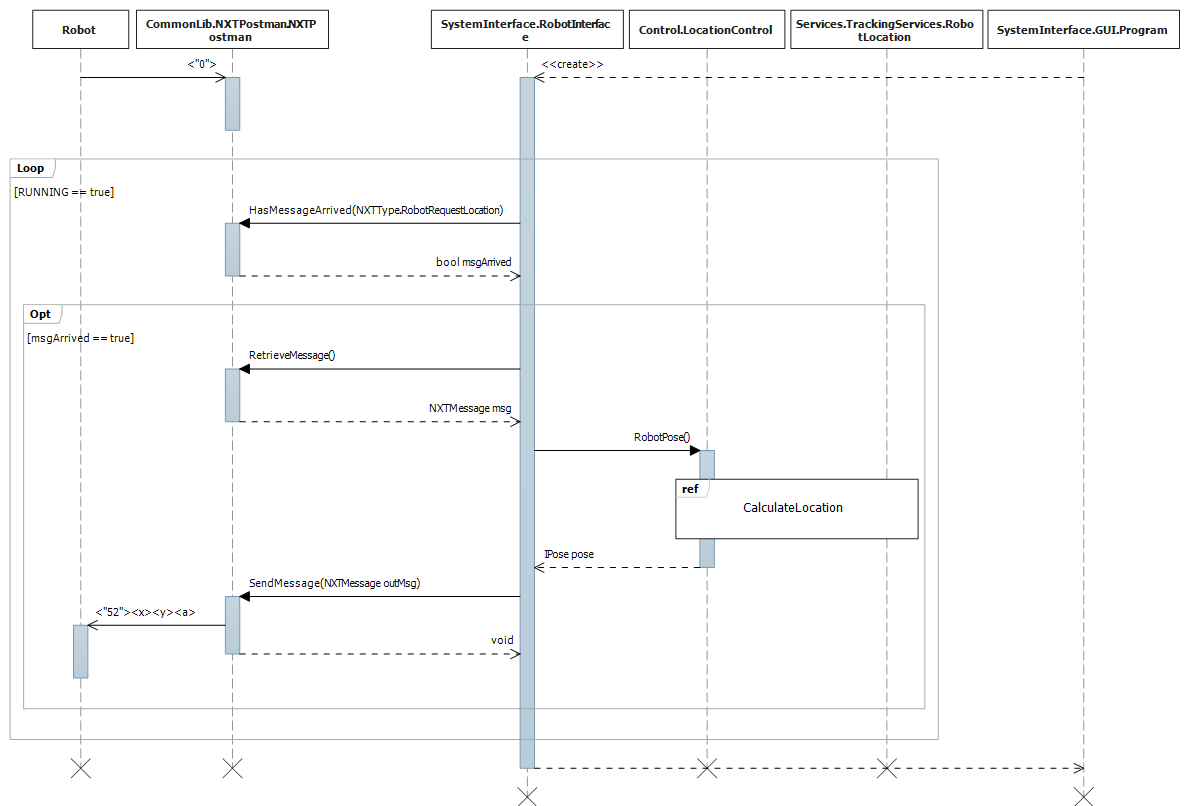
\includegraphics[width=\textwidth]{sdRequestLocation}
\caption{Sekvens-diagram for robottens anmodning om positur.}
\label{flow:ssd}
\end{figure}

\subsubsection{Robotten sender anmodning om sin positur}
Det første der sker er, at robotten lægger beskeden \lstinline[style=c]!OUTGOING_WHERE_AM_I! i \lstinline[style=c]!OUTBOX!:

\begin{lstlisting}[style=csmall,label=lst:whereami_request,caption=Robotten sender anmodning om positur.]
string msg = NumToStr(OUTGOING_WHERE_AM_I);
SendMessage(OUTBOX, msg);
\end{lstlisting}

Herefter går robotten i gang med kontinuerligt at checke \lstinline[style=c]!INBOX! indtil beskeden med typen \lstinline[style=c]!INCOMING_GET_POS! er at finde:

\begin{lstlisting}[style=csmall,label=lst:whereami_response,caption=Robotten venter på svar.]
while(true) {
   ReceiveRemoteString(INBOX, true, in);
   if (StrLen(in) > 0) {
      cmd = SubStr(in, 0, 2);
      cmdType = StrToNum(cmd);
      if (cmdType == INCOMING_GET_POS) {...} (*\label{whereami_request:if}*)
   }
}
\end{lstlisting}

\subsubsection{RobotInterface afventer besked fra robotten}
Håndtering af robottens beskeder/anmodninger sker i \lstinline[style=csharp]!RobotInterface!.
Her kører en seperat tråd med funktionen \lstinline[style=csharp]!listener()!:
\begin{lstlisting}[style=csharpsmall,label=lst:listener,caption=listener() i RobotInterface.]
private void listener()
{
    while (RUNNING)
    {
        if (checkForMessages()) (*\label{listener:checkformessages}*)
        {
            NXTMessage msg = postman.RetrieveMessage(); (*\label{listener:retrievemessage}*)

            switch (msg.MessageType)
            {
                case (NXTMessageType.RobotRequestsLocation):
                    RobotRequestLocation(); (*\label{listener:case}*)
                    break;
                //other cases
            }
        }
        Thread.Sleep(THREAD_SLEEP_INTERVAL_IN_MILLISECONDS);
    }
}
\end{lstlisting}

Tråden med \lstinline[style=csharp]!listener()! sættes i gang når PC programmet startes.

I \cref{listener:checkformessages} i \cref{lst:listener} kontrolleres det, om der findes besked i \lstinline[style=csharp]!PC_INBOX! af de indgående besked-typer:

\begin{lstlisting}[style=csharpsmall,label=lst:checkformessages,caption=checkForMessages() i RobotInterface.]
private bool checkForMessages()
{
    return postman.HasMessageArrived(NXTMessageType.RobotRequestsLocation)
        || postman.HasMessageArrived(NXTMessageType.RobotHasArrivedAtDestination);
}
\end{lstlisting}

Hvis der findes besked, hentes denne via \lstinline[style=csharp]!RetrieveMessage()! i \lstinline[style=csharp]!NXTPostman! (se \cref{listener:retrievemessage} i \cref{lst:listener}), som bruger Bluetooth-forbindelsen i \lstinline[style=csharp]!CommLink! til at checke efter nye beskeder på i robottens \lstinline[style=c]!OUTBOX!:

\begin{lstlisting}[style=csharpsmall,label=lst:postman,caption=RetrieveMessage i NXTPostman.]
public NXTMessage RetrieveMessage()
{
    try
    {
        byte[] msg = CommunicationBrick.CommLink.MessageReadToBytes(PC_INBOX, NxtMailbox.Box0, true);
        return new NXTMessage(msg);
    }
    catch {...}
}
\end{lstlisting}

Når beskeden \lstinline[style=csharp]!NXTMessageType.RobotRequestsLocation! findes i \lstinline[style=csharp]!PC_INBOX! (se \cref{listener:case} i \cref{lst:listener}) udføres den pågældende metode \lstinline[style=csharp]!RobotRequestLocation()!:

\begin{lstlisting}[style=csharpsmall,label=lst:robotrequestslocation,caption=RobotRequestsLocation() i RobotInterface.]
private void RobotRequestLocation()
{
    IPose pose = locCon.RobotPose; (*\label{robotrequestslocation:pose}*)
    string encodedMsg = NXTEncoder.Encode(pose);
    NXTMessage outMsg = new NXTMessage(NXTMessageType.SendPostion, encodedMsg);
    postman.SendMessage(outMsg); (*\label{robotrequestslocation:send}*)
}
\end{lstlisting}

\subsubsection{RobotInterface aflæser positur i LocationControl}
RobotInterface får den senest opdateret positur ved at aflæse en property på \lstinline[style=csharp]!LocationControl!.
Dette kan ses i \cref{robotrequestslocation:pose} i \cref{lst:robotrequestslocation}.

\subsubsection{LocationControl aflæser positur i TrackingServices}
LocationControl får den senest opdateret positur ved at aflæse en property i \lstinline[style=csharp]!TrackingServices!.
\lstinline[style=csharp]!TrackingServices! opdaterer sin nuværende viden om robottens positur løbende, ved kontinuerligt at beregne en ny ud fra Kinect'ens billede.

\subsubsection{RobotInterface bruger Postman til at sende positur}
RobotInterface har nu det seneste data om robottens positur.
Den bruger så \lstinline[style=csharp]!NXTPostman! (se \cref{robotrequestslocation:send} i \cref{lst:robotrequestslocation}) til at lægge beskeden (først encodes beskeden jf. \cref{protokol:positur}) af type \lstinline[style=csharp]!NXTMessageType.SendPosition! i \lstinline[style=csharp]!PC_OUTBOX!, som er robottens \lstinline[style=c]!INBOX!:

\begin{lstlisting}[style=csharpsmall,label=lst:sendmessage,caption=SendMessage i NXTPostman.]
public void SendMessage(NXTMessage msg)
{
    string toSendMessage = String.Format("{0}{1}", (byte)msg.MessageType, msg.EncodedMsg);
    CommunicationBrick.CommLink.MessageWrite(PC_OUTBOX, toSendMessage);
}
\end{lstlisting}

\subsubsection{Robotten modtager svar indeholdende den ny positur}
Robotten, som ventede på besked ved kontinuerligt at checke sin \lstinline[style=c]!INBOX!, har nu fået en besked af typen \lstinline[style=c]!INCOMING_GET_POS! og kan derved opdatere sin interne repræsentation af dens nuværende positur, som er kroppen af if-sætningen i \cref{whereami_request:if} i \cref{lst:whereami_request} (ikke vist).
